\documentclass[a4paper, 12pt]{article}
\usepackage[utf8x]{inputenc}
\usepackage{cmap}
\usepackage[english, russian]{babel}
\usepackage{indentfirst}
\usepackage[left=20mm, top=20mm, right=20mm, bottom=20mm]{geometry}
\usepackage{tikz}
\usepackage{float}
\usepackage{amsmath, amsfonts, amssymb}
\usepackage{graphicx}
\usepackage{fancybox, fancyhdr}
\usepackage{hyperref}
\usepackage{listings}
\usepackage{caption}
\usepackage{subcaption}
\usepackage{xcolor}
\pagestyle{fancy}
\fancyhf{}
\fancyhead[L]{Домашнее задание №2}
\fancyhead[R]{Теоретическая вероятность}
\fancyfoot[C]{\thepage}
\graphicspath{{images/}}
\usetikzlibrary{patterns}
\definecolor{LightGray}{gray}{0.95}
\definecolor{LightGray2}{gray}{0.7}
\lstdefinestyle{pycode}{
    language=Python,
    basicstyle=\footnotesize\ttfamily,
    numbers=left,
    numberstyle=\scriptsize\color{gray},
    stepnumber=1,
    numbersep=5pt,
    backgroundcolor=\color{LightGray},
    showspaces=false,
    showstringspaces=false,
    showtabs=false,
    tabsize=4,
    captionpos=b,
    breaklines=true,
    breakatwhitespace=false,
    frame=single,
    rulecolor=\color{LightGray2},
    linewidth=\linewidth,
    keywordstyle=\color{blue}\bfseries,
    commentstyle=\color{green!40!black},
    stringstyle=\color{purple},
    escapeinside={\%*}{*)},
    inputencoding=utf8x,
    xleftmargin=0pt,
    framexleftmargin=0pt,
    framexrightmargin=0pt
}
\lstset{style=pycode}
\hypersetup{
    colorlinks=true,
    linkcolor=blue,
    filecolor=magenta,
    urlcolor=cyan,
    pdftitle={contents setup},
    pdfpagemode=FullScreen,
}
\setlength{\parskip}{1.5mm}
\setlength{\headheight}{15pt}
\setlength{\footskip}{15pt}
\allowdisplaybreaks
\DeclareMathOperator{\sinc}{sinc}
\newcommand{\frc}[2]{\raisebox{2pt}{$#1$}\big/\raisebox{-3pt}{$#2$}}

\begin{document}
    \begin{titlepage}

        \begin{center}
        
\includegraphics[width=0.3\textwidth]{itmo.png} % requires itmo.png in /images folder
        \vfill

        Федеральное государственное автономное образовательное учреждение высшего образования
        «Национальный Исследовательский Университет ИТМО»\\

        \vfill
        {\large\bf ДОМАШНЕЕ ЗАДАНИЕ №2}\\
        {\large\bf ПРЕДМЕТ «ТЕОРЕТИЧЕСКАЯ ВЕРОЯТНОСТЬ»}\\
        Вариант №1
        \vfill

        \begin{flushright}
            \begin{minipage}{.45\textwidth}
            {
                \hbox{Преподаватель:}
                \hbox{Шиманская Г. С.}
                \hbox{Студент:}
                \hbox{Румянцев А. А.}
                \hbox{}
                \hbox{Номер ИСУ:}
                \hbox{368731}
                \hbox{Поток:}
                \hbox{ТеорВер 1.2}
                \hbox{Факультет:}
                \hbox{СУиР}
                \hbox{Группа:}
                \hbox{R3241}
            }
            \end{minipage}
        \end{flushright}

        \vfill

        Санкт-Петербург\\
        2024
        \end{center}
    \end{titlepage}

    \tableofcontents

    \newpage
    \section{Задание 1.}
    \subsection{Условие задачи.}
    В кармане имеется 3 монеты по 5 рублей, 2 монеты по 3 рубля и 6 монет 
    по рублю. Из кармана случайным образом извлекаются три монеты, 
    составить ряд распределения суммы вытащенных из кармана денег, 
    построить функцию распределения, найти мат. ожидание, дисперсию, 
    с.кв.откл., медиану, моду. Построить график функции распределения, 
    многоугольник распределения.


    \subsection{Решение.}
    Рассмотрим различные комбинации трех монет. Пока что не будем учитывать перестановки.
    $$
    555,\ 553,\ 551,\ 331,\ 111,\ 531,\ 533,\ 311,\ 511
    $$
    Запомним соответствующие им суммы.
    $$
    15,\ 13,\ 11,\ 7,\ 3,\ 9,\ 11,\ 5,\ 7
    $$


    Числа в каждой из комбинаций можно располагать в разном порядке. Например, пятерки
    и единицы можно расположить в строку из трех чисел шестью способами. Поэтому нам
    потребуется использовать формулу сочетаний из $n$ по $k$ вида
    $$
    C_n^k=\dfrac{n!}{(n-k)!\,k!};
    $$
    Распишем число сочетаний для каждой из комбинаций, приведенных ранее.
    $$
    C_3^3,\ C_3^2\cdot C_2^1,\ C_3^2\cdot C_6^1,\ C_2^2\cdot C_6^1,\ C_6^3,\ C_3^1\cdot C_2^1\cdot C_6^1,\ C_3^1\cdot C_2^2,\ C_2^1\cdot C_6^2,\ C_3^1\cdot C_6^2
    $$


    Чтобы найти вероятность с помощью перестановок нужно учесть все возможные исходы. Всего монет 11,
    а берем мы 3, значит для нахождения вероятности нам потребуется поделить число сочетаний для каждого
    рассматриваемого случая на
    $$
    C_{11}^3=\dfrac{11!}{(11-3)!\,3!}=165;
    $$
    Пример расчета приведен ниже.
    $$
    \dfrac{C_3^1\cdot C_2^1\cdot C_6^1}{C_{11}^3}=\dfrac{\dfrac{3!}{2!}\cdot\dfrac{2!}{1!}\cdot\dfrac{6!}{5!}}{165}=\dfrac{12}{55}
    $$


    Теперь составим ряд распределения суммы вытащенных из кармана денег.
    Ранее мы записывали ее для каждой из комбинаций. Видим, что сумма в 7 и 11 рублей повторяются дважды --
    вероятность для этих сумм будет складываться из соответствующих вероятностей, посчитанных формулой сочетаний.
    Получим следующее:
    $$
    P(X=7)=\dfrac{C_2^2\cdot C_6^1}{C_{11}^3}+\dfrac{C_3^1\cdot C_6^2}{C_{11}^3}=\dfrac{2}{55}+\dfrac{3}{11}=\dfrac{17}{55}
    $$
    $$
    P(X=11)=\dfrac{C_3^2\cdot C_6^1}{C_{11}^3}+\dfrac{C_3^1\cdot C_2^2}{C_{11}^3}=\dfrac{6}{55}+\dfrac{1}{55}=\dfrac{7}{55}
    $$


    \newpage
    Теперь составим таблицу $p_i(x_i)$.
    \begin{table}[h]
        \centering
        \begin{tabular}{|c|c|c|c|c|c|c|c|}
        \hline
        $x_i$ & 3 & 5 & 7 & 9 & 11 & 13 & 15 \\
        \hline
        $p_i$ & $\frc{4}{33}$ & $\frc{2}{11}$ & $\frc{17}{55}$ & $\frc{12}{55}$ & $\frc{7}{55}$ & $\frc{2}{55}$ & $\frc{1}{165}$ \\
        \hline
        \end{tabular}
        \caption{Ряд распределения суммы вытащенных из кармана денег.}
        \label{tab:moneysum}
    \end{table}


    Запишем функцию распределения $F(x)$, построим ее график и многоугольник распределения.
    $$F(x)=
    \begin{cases}
        0, & x\leq 3\\
        \frc{4}{33}, & 3 < x \leq 5\\
        \frc{10}{33}, & 5 < x \leq 7\\
        \frc{101}{165}, & 7 < x \leq 9\\
        \frc{137}{165}, & 9 < x \leq 11\\
        \frc{158}{165}, & 11 < x \leq 13\\
        \frc{164}{165}, & 13 < x \leq 15\\
        1, & x > 15
    \end{cases}
    $$
    \begin{figure}[H]
        \centering
        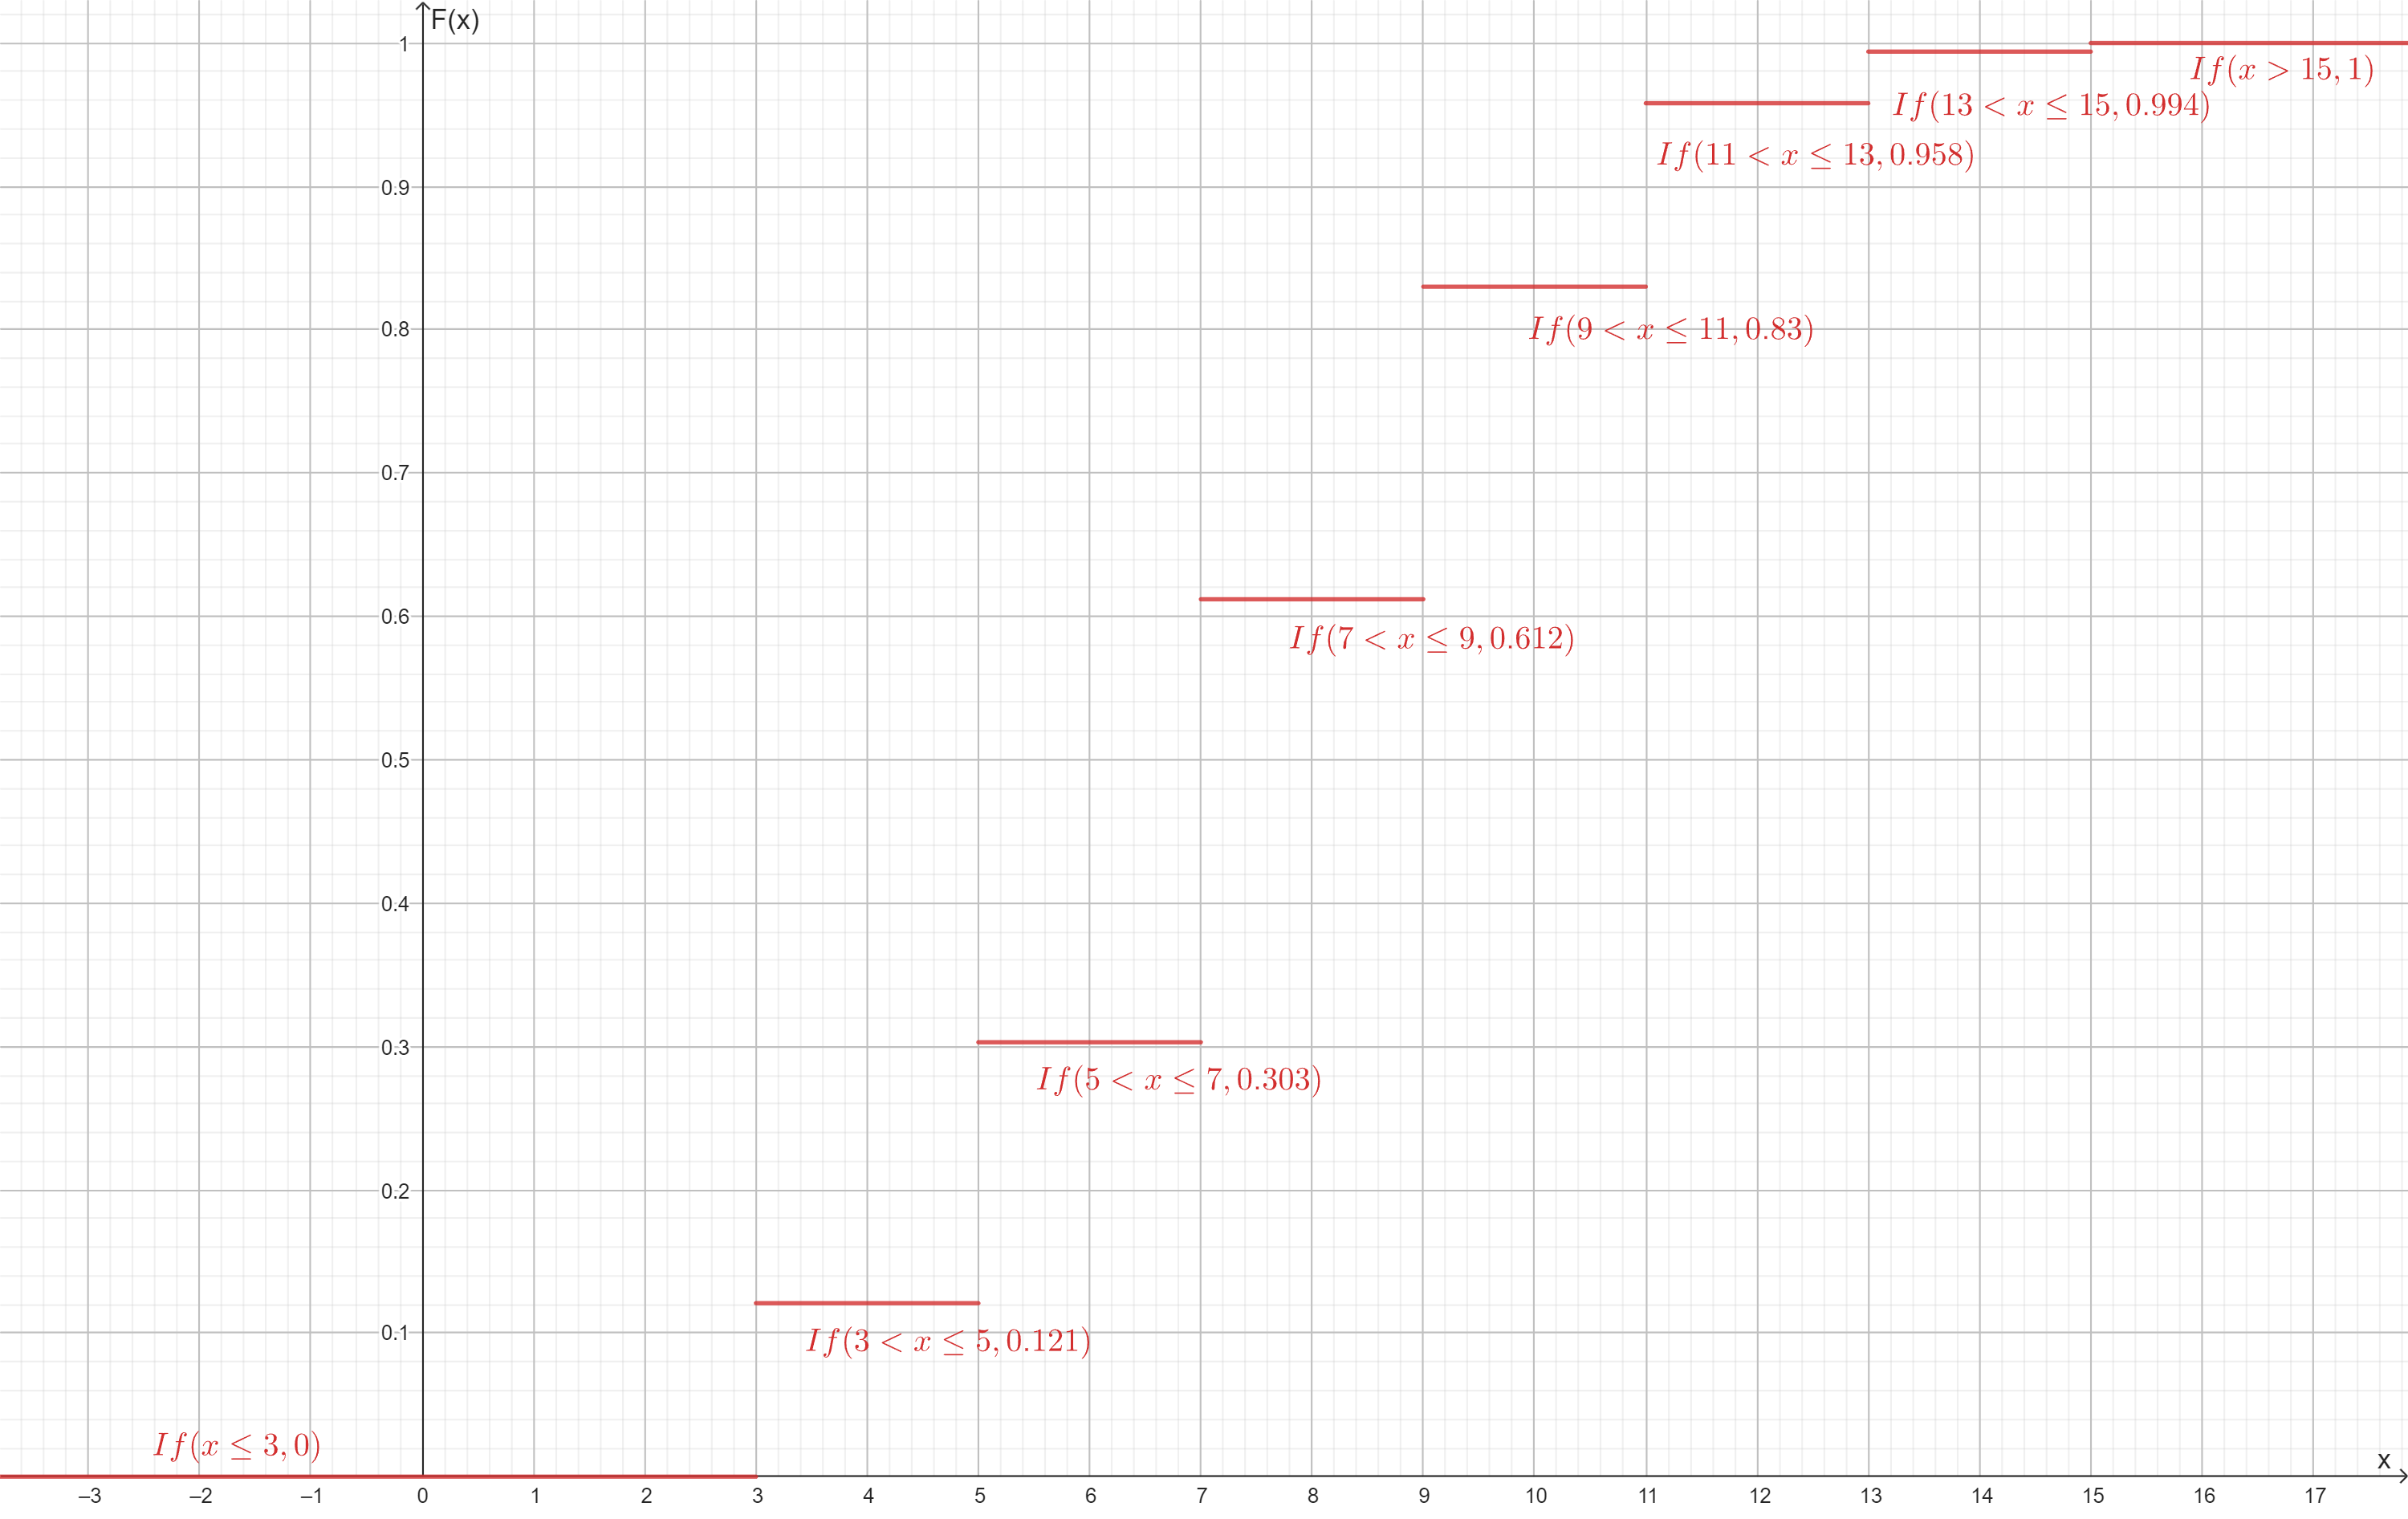
\includegraphics[scale=0.5]{F_x.png}
        \captionsetup{skip=0pt}
        \caption{График функции распределения.}
        \label{fig:F_x}
    \end{figure}
    \begin{figure}[H]
        \centering
        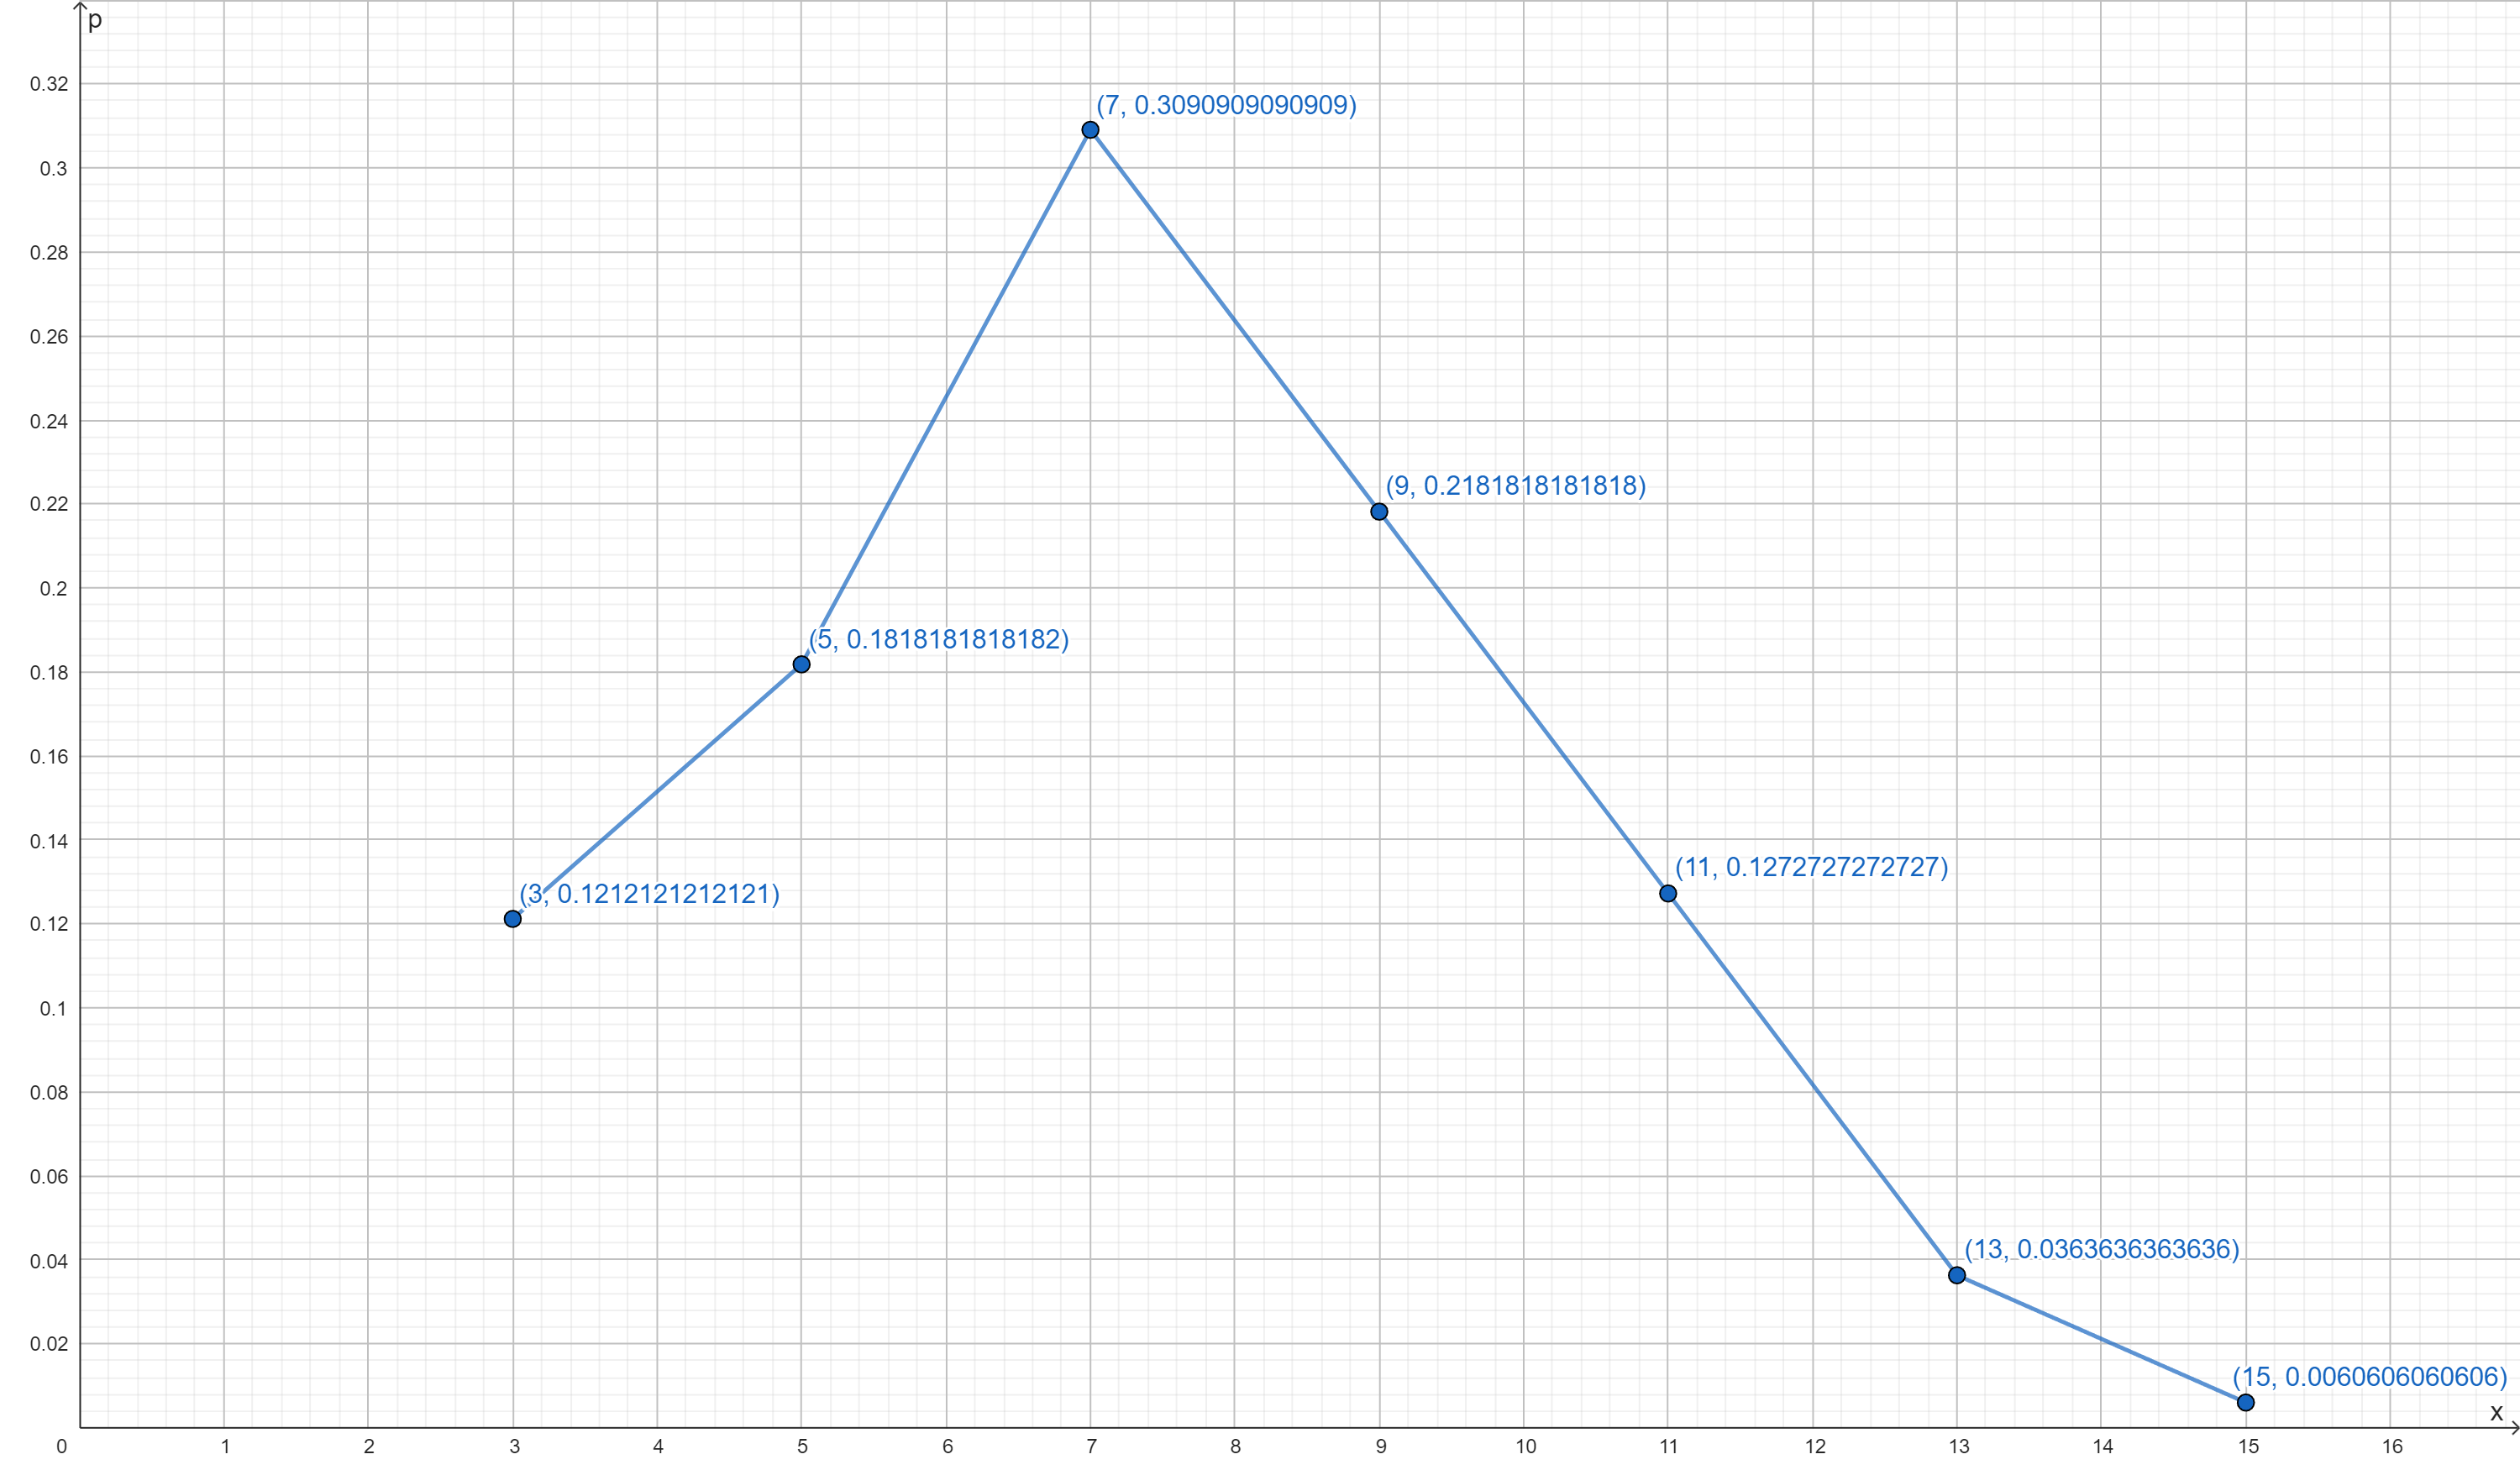
\includegraphics[scale=0.65]{polydis.png}
        \captionsetup{skip=0pt}
        \caption{Многоугольник распределения.}
        \label{fig:polydis}
    \end{figure}


    \newpage
    Далее найдем математическое ожидание ($k$ -- количество $x_i$), дисперсию, среднеквадратичное отклонение, медиану, моду и вероятность того,
    что сумма окажется не менее 10 рублей. Медиана -- средний элемент выборки, левее и правее которого одинаковое количество элементов,
    если в выборке нечетное количество значений. Мода -- самый часто повторяющийся элемент выборки. В нашем случае их два, поэтому я приведу оба.
    $$
    M(x)=\sum\limits_{i=1}^kx_ip_i=3\cdot\dfrac{4}{33}+5\cdot\dfrac{2}{11}+7\cdot\dfrac{17}{55}+9\cdot\dfrac{12}{55}+11\cdot\dfrac{7}{55}+13\cdot\dfrac{2}{55}+15\cdot\dfrac{1}{165}=\dfrac{81}{11},
    $$
    $$
    M(x^2)=\sum\limits_{i=1}^kx_i^2p_i=3^2\cdot\dfrac{4}{33}+5^2\cdot\dfrac{2}{11}+7^2\cdot\dfrac{17}{55}+9^2\cdot\dfrac{12}{55}+11^2\cdot\dfrac{7}{55}+13^2\cdot\dfrac{2}{55}+15^2\cdot\dfrac{1}{165}=\dfrac{675}{11},
    $$
    $$
    D(x)=M(x^2)-(M(x))^2=\dfrac{675}{11}-\left(\dfrac{81}{11}\right)^2=\dfrac{675}{11}-\dfrac{6561}{121}=\dfrac{864}{121},
    $$
    $$
    \delta(x)=\sqrt{D(x)}=\sqrt{\dfrac{864}{121}}=\dfrac{12\sqrt{6}}{11},
    $$
    $$
    MED(x)=9\Rightarrow P(X=MED(x)=9)=\dfrac{12}{55},
    $$
    $$
    MODE_1(x)=7\Rightarrow P(X=MODE_1(x)=7)=\dfrac{17}{55},
    $$
    $$
    MODE_2(x)=11\Rightarrow P(X=MODE_2(x)=11)=\dfrac{7}{55},
    $$
    $$
    P(X\geq 10)=P(X=11)+P(X=13)+P(X=15)=\dfrac{7}{55}+\dfrac{2}{55}+\dfrac{1}{165}=\dfrac{28}{165}
    $$


    \begin{align*}
        & \textbf{Ответ:}\\
        & \mathbf{M(X)=\dfrac{81}{11},\ D(X)=\dfrac{864}{121},\ \delta(X)=\dfrac{12\sqrt{6}}{11}}, \ \mathbf{P(X=MED(x)=9)=\dfrac{12}{55}}, \\
        & \mathbf{P(X=MODE_1(x)=7)=\dfrac{17}{55},\ P(X=MODE_2(x)=11)=\dfrac{7}{55},}\\ & \mathbf{P(X\geq 10)=\dfrac{28}{165}}
    \end{align*}


    \section{Задание 2.}
    \subsection{Условие задачи.}
    На рынок поступила партия арбузов. Предполагается, что вес одного 
    арбуза -- случайная величина, подчиняющаяся нормальному закону 
    распределения с математическим ожиданием $M(X) = 9$ кг и средним 
    квадратическим отклонением $\sigma = 0.5$ кг. Определите вероятность того, 
    что вес случайно отобранного арбуза:
    \begin{enumerate}
        \item Окажется больше 12 кг;
        \item Окажется меньше 7.5 кг;
        \item Будет находиться между 8.5 и 9.5 кг;
        \item Отклонится от математического ожидания меньше, чем на 0.1 кг;
        \item Отклонится от математического ожидания больше, чем на 0.2 кг;
    \end{enumerate}
    6. Найдите границы, в которых отклонение веса случайно отобранной 
    туши от своего математического ожидания не превысит утроенного среднего 
    квадратического отклонения (проиллюстрируйте правило трех сигм).


    \subsection{Решение.}
    Запомним важные данные -- мат. ожидание $M(X)=9$ кг и ср. кв. откл. $\sigma=0.5$ кг.


    Для первого задания отклонение $\mu=12$ кг. Сначала найдем вероятность, что масса арбуза
    окажется меньше 12 кг (значения $\Phi$ смотрим по таблице в интернете):
    $$
    P(X\leq Z)=\Phi\left(\dfrac{\mu-M(X)}{\sigma}\right)=\Phi\left(\dfrac{12-9}{0.5}\right)=\Phi\left(6\right)=P(X\leq Z=6)\approx 1
    $$


    Получили площадь под графиком нормального распределения вплоть до $6\sigma$.
    Чтобы найти обратную вероятность (масса арбуза окажется больше 12 кг), вычтем из 1 полученную вероятность
    на предыдущем шаге:
    $$
    P=1-P(X\leq Z=6)=1-1=0
    $$
    Как видим, вероятность такого отклонения стремится к нулю, что логично, так как площадь за $6\sigma$ стремится к 0,
    а мы нашли все, что до нее, площадь чего стремится к 1.


    Для второго задания $\mu=7.5$ кг. От нас требуют найти площадь под графиком нормального распределения в
    диапазоне $[-\infty,7.5]$. Мы сразу можем найти соответствующую вероятность (вычисления с $\Phi$ аналогичные):
    $$
    P=\Phi\left(\dfrac{7.5-9}{0.5}\right)=\Phi(-3)=0.0135
    $$
    Вероятность получилась очень маленькой, что означает, что площадь нормального распределения от 7.5 до $-\infty$ кг
    стремится к нулю.


    В третьем задании необходимо найти площадь средней части нормального распределния при $\mu_1=8.5,\,\mu_2=9.5$ кг.
    Аналогично найдем вероятность. Вычтем из площади от $-\infty$ до 9.5 площадь $-\infty$ до 8.5 кг и получим середину:
    $$
    P=\Phi\left(\dfrac{9.5-9}{0.5}\right)-\Phi\left(\dfrac{8.5-9}{0.5}\right)=\Phi(1)-\Phi(-1)=0.84134-0.15866=0.68268
    $$
    Здесь вероятность получилась уже побольше, что логично, так как средняя часть нормального распределения имеет явно б\'{о}льшую
    площадь, чем ее края.


    В четвертом задании все то же самое, но теперь отклонение задано как $M(X)<0.1$ кг.
    $$
    P=\Phi\left(\dfrac{9.1-9}{0.5}\right)-\Phi\left(\dfrac{8.9-9}{0.5}\right)=\Phi(0.2)-\Phi(-0.2)=0.57926-0.4274=0.15186
    $$
    Вероятность получилась небольшой, так как мы взяли лишь малую часть площади средней части нормального распределения.


    В пятом задании отклонение задано как $M(X)>0.2$ кг. Функция нормального распределения является симметричной.
    Значит нам достаточно посчитать только часть левее середины, которая при стремлении к $-\infty$ стремится к 0,
    и умножить на 2.
    $$
    P=2\Phi\left(\dfrac{8.8-9}{0.5}\right)=2\Phi(-0.4)=2\cdot 0.34458=0.68916
    $$


    Для последнего задания нужно решить систему, чтобы определить границы, в которых отклонение веса случайно
    отобранной туши от своего мат. ожидания не превысит $3\sigma$.
    \begin{align*}
    \Phi\left(\dfrac{x-9}{0.5}\right)=
    \begin{cases}
        \frc{(x-9)}{0.5}\geq -3\\
        \frc{(x-9)}{0.5}\leq 3
    \end{cases}\
    \Phi\left(\dfrac{x-9}{0.5}\right)=
    \begin{cases}
        x\geq 7.5\\
        x\leq 10.5
    \end{cases}
    \end{align*}
    Получили диапазон $[7.5,10.5]$. Теперь проиллюстрируем правило трех сигм -- разница $\Phi$ в этом
    диапазоне должна быть равна примерно 0.997:
    $$
    P=\Phi\left(\dfrac{10.5-9}{0.5}\right)-\Phi\left(\dfrac{7.5-9}{0.5}\right)=\Phi\left(3\right)-\Phi\left(-3\right)=0.99865-0.00135=0.9973
    $$
    Видим, что правило трех сигм выполняется.


    \begin{align*}
        & \textbf{Ответ:}\\
        & \mathbf{1.\,P\approx0,\ 2.\,P=0.0135,\ 3.\,P=0.68268,}\\
        & \mathbf{4.\,P=0.15186,\ 5.\,P=0.68916,\ 6.\,[7.5,10.5]}
    \end{align*}


    \section{Задание 3.}
    \subsection{Условие задачи.}
    В урне 5 шаров: 3 белых и 2 черных. Производится две
    последовательных выборки без возвращения каждый раз по два шара.
    Определены две случайные величины: число белых шаров в первой
    выборке и число белых шаров во второй выборке. Построить функцию
    распределения, ее график.


    \subsection{Решение.}
    Пусть $X$ -- число \textit{белых шаров}, полученных в первую выборку, $Y$ -- во вторую.
    Функция плотности распределения будет выглядеть как таблица, где столбец будет отвечать за
    $X$, строка -- за $Y$. Рассматривать нужно случаи 0, 1, 2 -- достали 0 белых шаров, 1 и 2
    соответственно.


    Теперь поочередно будем рассматривать элементы таблицы. Будем представлять их в
    виде -- $a_{ij}$ -- элемент $a$ на $i$ строке и $j$ столбце. Счет строк и столбцов начинается с нуля, как
    в программировании. Для определения вероятности будем пользоваться формулой числа сочетаний из $n$ по $k$.
    Если, например, $i=1$, $j=1$, то это означает, что в первую выборку достали 1 белый шар и 1 черный, во вторую
    то же самое. Для нахождения вероятности каждого случая, необходимо делить результат сочетаний на
    $$
    C_5^2=\dfrac{5!}{2!\,3!}=10,\ C_3^2=\dfrac{3!}{2!}=3,
    $$
    где $C_5^2$ -- достали 2 шара из 5, $C_3^2$ -- достали 2 шара из 3 (два уже взяли, шары не возвращаются).
    Таким образом, получим:
    \begin{align*}
        & a_{00}=0\ \text{(Не хватит черных шаров, в этом случае нужно 4, а их 2)}\\
        & a_{22}=0\ \text{(Не хватит белых шаров, в этом случае нужно 4, а их 3)}\\
        & a_{10}=0\ \text{(Не хватит черных шаров, в этом случае нужно 3, а их 2)}\\
        & a_{01}=0\ (\text{Аналогично элементу } a_{10})\\
        & a_{02}=\dfrac{C_3^0\,C_2^2}{C_5^2}\cdot\dfrac{C_3^2}{C_3^2}=\dfrac{\frc{3!}{3!}\cdot\frc{2!}{2!}}{10}=0.1\\
        & a_{20}=\dfrac{C_3^2\,C_2^0}{C_5^2}\cdot\dfrac{C_1^0\,C_2^2}{C_3^2}=\dfrac{\frc{3!\,2!}{2!\,2!}}{10}\cdot\dfrac{\frc{1!\,2!}{1!\,2!}}{3}=0.1\\
        & a_{11}=\dfrac{C_3^1\,C_2^1}{C_5^2}\cdot\dfrac{C_2^1\,C^1_1}{C_3^2}=\dfrac{\frc{3!\,2!}{2!\,1!}}{10}\cdot\dfrac{\frc{2!\,1!}{1!\,1!}}{3}=0.4\\
        & a_{21}=\dfrac{C_3^2\,C_2^0}{C_5^2}\cdot\dfrac{C_1^1\,C_2^1}{C_3^2}=\dfrac{\frc{3!\,2!}{2!\,2!}}{10}\cdot\dfrac{\frc{1!\,2!}{1!\,1!}}{3}=0.2\\
        & a_{12}=\dfrac{C_3^1\,C^1_2}{C^2_5}\cdot\dfrac{C^2_2\,C^0_1}{C^2_3}=\dfrac{\frc{3!\,2!}{2!}}{10}\cdot\dfrac{\frc{2!\,1!}{2!\,1!}}{3}=0.2
    \end{align*}


    Теперь составим таблицу функции плотности распределения $f(x,y)$.
    \begin{table}[h]
        \centering
        \begin{tabular}{|c|c|c|c|}
        \hline
        $x \text{\textbackslash} y$ & 0 & 1 & 2 \\
        \hline
        0 & 0 & 0 & 0.1\\
        \hline
        1 & 0 & 0.4 & 0.2\\
        \hline
        2 & 0.1 & 0.2 & 0\\
        \hline
        \end{tabular}
        \caption{Функция плотности распределения $f(x,y)$.}
        \label{tab:f_x}
    \end{table}


    Осталось составить таблицу функции распределения и построить ее график. Здесь вместо 0, 1, 2 будут
    следующие строки и столбцы соответственно: $x\leq 0$, $0<x\leq1$, $1<x\leq2$, $x>2$ и $y\leq 0$, $0<y\leq1$, $1<y\leq2$, $y>2$.
    Для построения таблицы нужно рассмотреть все эти случаи совместно. Элементы расписаны аналогично предыдущей таблице.
    Пользоваться будем следующей формулой: $$F(x,y)=P(X<x,Y<x);$$
    Теперь найдем все элементы по ней.
    \begin{align*}
        & x\leq 0,\,y\leq0\Rightarrow a_{00}=F(x,y)=P(X<0,Y<0)=0,\\
        & 0<x\leq 1,\,y\leq0\Rightarrow a_{10}=F(x,y)=P(X<1,Y<0)=0,\\
        & 1<x\leq 2,\,y\leq0\Rightarrow a_{20}=F(x,y)=P(X<2,Y<0)=0,\\
        & x>2,\,y\leq0\Rightarrow a_{30}=F(x,y)=P(X=0,1,2;Y<0)=0,\\
        & \text{Для диапазонов } y \text{ аналогично, так как } \nexists\,X<0,\\
        & 0<x\leq1,\,0<y\leq1\Rightarrow a_{11}=F(x,y)=P(X<1,Y<1)=0,\\
        & 0<x\leq1,\,1<y\leq2\Rightarrow a_{12}=F(x,y)=P(X<1,Y<2)=0+0=0,\\
        & 0<x\leq1,\,y>2\Rightarrow a_{13}=F(x,y)=P(X=0;Y=0,1,2)=0+0+0.1=0.1,\\
        & 1<x\leq2,\,0<y\leq1\Rightarrow a_{21}=F(x,y)=P(X=0,1;Y=0)=0+0=0,\\
        & x>2,\,0<y\leq1\Rightarrow a_{31}=F(x,y)=P(X=0,1,2;Y=0)=0+0+0.1=0.1,\\
        & 1<x\leq2,\,1<y\leq2\Rightarrow a_{22}=F(x,y)=P(X=0,1;Y=0,1)=0+0+0+0.4,\\
        & x>2,\,1<y\leq2\Rightarrow a_{32}=F(x,y)=P(X=0,1,2;Y=0,1)=0.4+0.1+0.2=0.7,\\
        & 1<x\leq2,\,y>2\Rightarrow a_{23}=F(x,y)=P(X=0,1;Y=0,1,2)=0.4+0.1+0.2=0.7,\\
        & x>2,\,y>2\Rightarrow a_{33}=F(x,y)=P(X=0,1,2;Y=0,1,2)=0.1+0.4+0.2+0.1+0.2=1
    \end{align*}


    Результаты приведены ниже:
    \begin{table}[h]
        \centering
        \begin{tabular}{|c|c|c|c|c|}
        \hline
        $x \text{\textbackslash} y$ & $y\leq0$ & $0<y\leq1$ & $1<y\leq2$ & $y>2$ \\
        \hline
        $x\leq0$ & 0 & 0 & 0 & 0\\
        \hline
        $0<x\leq1$ & 0 & 0 & 0 & 0.1\\
        \hline
        $1<x\leq2$ & 0 & 0 & 0.4 & 0.7\\
        \hline
        $x>2$ & 0 & 0.1 & 0.7 & 1\\
        \hline
        \end{tabular}
        \caption{Функция распределения $F(x,y)$.}
        \label{tab:F_x}
    \end{table}
    \begin{figure}[H]
        \centering
        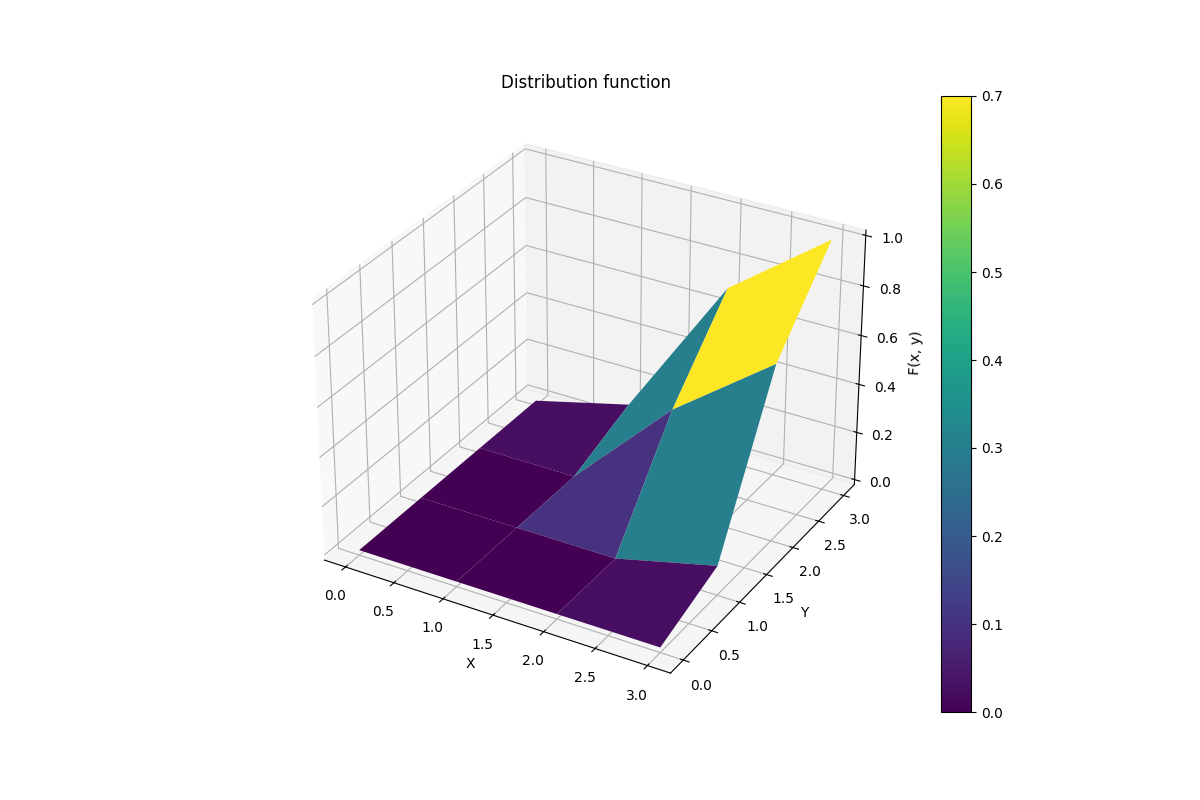
\includegraphics[scale=0.5]{disf.png}
        \captionsetup{skip=0pt}
        \caption{График функции распределения $F(x,y)$.}
        \label{fig:F_xg}
    \end{figure}


    \subsection{Листинг для задания 3.}
    Для построения трехмерного графика я написал код на языке Python с использованием библиотек
    numpy и matplotlib.
    \begin{lstlisting}[label=code, caption=Программа для построения трехмерного графика.]
    import matplotlib.pyplot as plt
    import numpy as np

    x = np.array([0, 1, 2, 3])
    y = np.array([0, 1, 2, 3])
    X, Y = np.meshgrid(x, y)
    Z = np.array([
        [0, 0, 0, 0],
        [0, 0, 0, 0.1],
        [0, 0, 0.4, 0.7],
        [0, 0.1, 0.7, 1]
    ])

    fig = plt.figure(figsize=(12, 8))
    ax = fig.add_subplot(111, projection='3d')

    surface = ax.plot_surface(X, Y, Z, cmap='viridis')

    fig.colorbar(surface)

    ax.set_title('Distribution function')
    ax.set_xlabel('X')
    ax.set_ylabel('Y')
    ax.set_zlabel('F(x, y)')
    ax.set_zlim(0, 1)

    plt.show()
    \end{lstlisting}


    \textbf{Ответ: Получена функция распределения F(x, y) и построен ее график.}


    \section{Задание 4.}
    \subsection{Условие задачи.}
    По данным статистической службы 7.5\% населения -- безработные.
    Используя неравенство Чебышева оценить вероятность того, что в
    наудачу отобранной группе в 1000 человек доля безработных заключена
    в границах от 4\% до 6\%. Найти вероятность того же события, используя
    следствие из интегральной теоремы Муавра-Лапласа. Сравнить
    результаты и обосновать их


    \subsection{Решение.}
    Для начала рассмотрим неравенство Чебышева. Пусть $X$ -- количество безработных в наудачу отобранной
    группе из $n=1000$ человек. Вероятность того, что человек безработный, дана в условии, и равна $p=0.075$.
    $X$ имеет биноминальное распределение вида
    $$
    X\sim Bin(1000, 0.075);
    $$
    Матожидание и дисперсия примут вид
    $$
    M(X)=np=1000\cdot0.075=75,
    $$
    $$
    D(X)=np(1-p)=1000\cdot0.075\cdot0.925=69.375
    $$


    Пусть $Y$ -- доля безработных в группе. Рассмотрим $Y$ и найдем для него матожидание, дисперсию и
    среднеквадратичное отклонение:
    $$
    Y=\dfrac{X}{1000},\ M(Y)=\dfrac{M(X)}{1000}=0.075,\ D(Y)=\dfrac{D(X)}{1000^2}=\dfrac{69.375}{1000000}=0.000069375,
    $$
    $$
    \sigma_{Y}=\sqrt{D(Y)}=\sqrt{0.000069375}\approx 0.00833;
    $$
    По неравенству Чебышева имеем:
    $$
    P(|Y-M(Y)|\geq k\sigma_{Y})\leq \dfrac{1}{k^2}
    $$
    По условию даны границы в 4\% и 6\%, рассмотрим $Y$ с отклонением в $7.5\%$:
    \begin{align*}
    0.04\leq& Y\leq 0.06\\
    0.04-0.075\leq& Y-0.075\leq 0.06-0.075\\
    -0.035\leq& Y-0.075\leq -0.015
    \end{align*}
    Выразим в единицах стандартного отклонения:
    $$
    -0.035\leq Y-0.075\leq -0.015\Rightarrow -\dfrac{0.035}{0.00833}\leq \dfrac{Y-0.075}{0.00833}\leq -\dfrac{0.015}{0.00833}\Rightarrow
    -4.2\leq k \leq -1.8
    $$
    Вернемся к неравенству Чебышева и подставим полученные значения:
    $$
    P(|Y-0.075|\geq 0.035)\leq \dfrac{1}{4.2^2}\approx 0.0566
    $$
    Тогда вероятность того, что доля безработных окажется в пределах от 4\% до 6\%:
    $$
    P(0.04\leq Y\leq 0.06)\geq 1-0.0566=0.9434
    $$


    Теперь найдем ту же вероятность, используя следствие из интегральной теоремы\\ Муавра-Лапласа --
    при большом $n$ можно использовать нормальное приближение вида
    $$
    X\approx\mathcal{N}\left(np,\sqrt{np(1-p)}\right)
    $$
    Применим его к $Y$:
    $$
    Y\approx \mathcal{N}\left(p,\sqrt{\dfrac{p(1-p)}{n}}\right)
    \Rightarrow Y\approx \mathcal{N}\left(0.075,\sqrt{\dfrac{0.075\cdot0.925}{1000}}\right)=\mathcal{N}(0.075,0.00833)
    $$
    Найдем вероятность того, что $Y$ находится в пределах 4\% и 6\%:
    $$
    P(0.04\leq Y\leq 0.06)=P\left(\dfrac{0.04-0.075}{0.00833}\leq Z \leq \dfrac{0.06-0.075}{0.00833}\right)
    =P(-4.2\leq Z\leq -1.8),
    $$
    где полученное $P(Z)$ -- стандартное нормальное распределение $Z$.
    Найдем для него значения:
    $$
    P(Z\leq -1.8)\approx 0.0359,\ P(Z\leq -4.2)\approx 0.000013
    $$
    Тогда имеем:
    $$
    P(-4.2 \leq Z \leq -1.8) = P(Z \leq -1.8) - P(Z \leq -4.2) \approx 0.0359 - 0.000013 = 0.0359
    $$
    Вероятность $P(Z\leq -4.2)$ очень мала, поэтому мы пренебрежем ей и получим
    ответ:
    $$
    P(-4.2\leq Z \leq -1.8)\approx0.0359\Rightarrow P(0.04\leq Y \leq 0.06)\approx0.0359
    $$


    По неравенству Чебышева вероятность того, что доля безработных окажется в пределах от 4\% до 6\% составила примерно 
    0.9434. По интегральной теореме Муавра-Лапласа вероятность составила примерно 0.0359.


    Неравенство Чебышева даёт менее точную оценку, так как оно применимо к любым распределениям и предоставляет верхнюю границу вероятности.
    В то время как теорема Муавра-Лапласа основана на нормальном приближении и даёт более точную оценку для больших выборок.

    Результаты отличаются, и оценка по теореме Муавра-Лапласа более точна в данном контексте из-за нормального распределения,
    которое лучше отражает реальное поведение биномиального распределения при больших $n$.


    \textbf{Ответ: что и требовалось исследовать.}


    \section{Задание 5.}
    \subsection{Условие задачи.}
    Вычислить характеристическую функцию и найти $M(X)$ и $D(X)$ для
    гипергеометрического распределения.


    \subsection{Решение.}
    Гипергеометрическое распределение описывает вероятность $X$ успехов в $n$ выборках без возвращения из конечной совокупности из
    $N$ элементов, содержащих $K$ успешных и $N-K$ неуспешных элементов. Будем обозначать гипергеометрическое распределение как
    $$X\sim \text{Hypergeometric}(N,K,n)$$
    Функция вероятности для гипергеометрического распределения имеет вид:
    $$
    P(X=k)=
    \dfrac{
        \begin{bmatrix}
            K\\
            k
        \end{bmatrix}
        \begin{bmatrix}
            N-K\\
            n-k
        \end{bmatrix}
    }{
        \begin{bmatrix}
            N\\
            n
        \end{bmatrix}
    },
    $$
    где
    $
    \begin{bmatrix}
        a\\
        b
    \end{bmatrix}
    $
    -- биномиальный коэффициент, равный
    $
    \dfrac{a!}{(a-b)!\,b!}
    $


    Чтобы найти характеристическую функцию, необходимо вычислить математическое ожидание от $e^{itX}$,
    где $i$ -- мнимая единица, а $t$ -- вещественное число.
    Характеристическая функция $\varphi_X(t)$ для случайной величины $X$ определяется как:
    $$
    \varphi_X(t)=M\left[e^{itX}\right]
    $$
    Для гипергеометрического распределения имеем:
    $$
    \varphi_X(t)=M\left[e^{itX}\right]=\sum\limits_{k=0}^{n}e^{itk}P(X=k)
    $$
    Ранее мы выписали функцию вероятности $P(X=k)$. Подставим ее в выражение выше:
    $$
    \varphi_X(t)=\sum\limits_{k=0}^{n}e^{itk}\dfrac{
        \begin{bmatrix}
            K\\
            k
        \end{bmatrix}
        \begin{bmatrix}
            N-K\\
            n-k
        \end{bmatrix}
    }{
        \begin{bmatrix}
            N\\
            n
        \end{bmatrix}
    }
    =\dfrac{1}{
        \begin{bmatrix}
            N\\
            n
        \end{bmatrix}
    }
    \sum\limits_{k=0}^{n}e^{itk}
    \begin{bmatrix}
        K\\
        k
    \end{bmatrix}
    \begin{bmatrix}
        N-K\\
        n-k
    \end{bmatrix}
    $$
    Для дальнейших вычислений будем использовать метод производящих функций. Пусть $G(z)$
    -- производящая функция для гипергеометрического распределения:
    $$
    G(z)=\sum\limits_{k=0}^{n}P(X=k)z^k
    $$
    Известно, что производящую функцию гипергеометрического распределения можно записать как:
    $$
    G(z)=\dfrac{
        \begin{bmatrix}
            N-n\\
            K
        \end{bmatrix}
    }{
        \begin{bmatrix}
            N\\
            K
        \end{bmatrix}
    }
    (1+(z-1))^n
    $$
    Чтобы получить характеристическую функцию, заменим $z$ на $e^{it}$:
    $$
    \varphi_X(t)=G(e^{it})=\dfrac{
        \begin{bmatrix}
            N-n\\
            K
        \end{bmatrix}
    }{
        \begin{bmatrix}
            N\\
            K
        \end{bmatrix}
    }(1+(e^{it}-1))^n
    $$
    Подставим это выражение в производящую функцию и получим окончательный вид характеристической функции гипергеометрического распределения:
    $$
    \varphi_X(t)=\dfrac{
        \begin{bmatrix}
            N-n\\
            K
        \end{bmatrix}
    }{
        \begin{bmatrix}
            N\\
            K
        \end{bmatrix}
    }(e^{it})^n
    =\dfrac{
        \begin{bmatrix}
            N-n\\
            K
        \end{bmatrix}
    }{
        \begin{bmatrix}
            N\\
            K
        \end{bmatrix}
    }e^{itn}
    $$
    Таким образом, характеристическая функция гипергеометрического распределения $X$ записывается так:
    $$
    \varphi_X(t)=
    \dfrac{
        \begin{bmatrix}
            N-n\\
            K
        \end{bmatrix}
    }{
        \begin{bmatrix}
            N\\
            K
        \end{bmatrix}
    }(1+(e^{it}-1))^n
    $$


    Математическое ожидание $M(X)$ можно получить как первую производную характеристической функции по $t$ при $t=0$:
    $$
    M[X]=\dfrac{d\varphi_X(t)}{dt}\bigg|_{t=0}
    $$
    Для гипергеометрического распределения получим:
    $$
    \dfrac{d\varphi_X(t)}{dt}\bigg|_{t=0}=
    \left(\dfrac{\begin{bmatrix}N-n\\K\end{bmatrix}}{\begin{bmatrix}N\\K\end{bmatrix}}(1+(e^{it}-1))^n\right)^{\prime}_t \Bigg|_{t=0}=
    \dfrac{
        \begin{bmatrix}
            N-n\\
            K
        \end{bmatrix}
    }{
        \begin{bmatrix}
            N\\
            K
        \end{bmatrix}
    }
    \cdot n \cdot (1+(e^{it}-1))^{n-1}\cdot ie^{it}\Bigg|_{t=0}
    $$
    $$
    \dfrac{d\varphi_X(t)}{dt}\bigg|_{t=0}=
    \dfrac{
        \begin{bmatrix}
            N-n\\
            K
        \end{bmatrix}
    }{
        \begin{bmatrix}
            N\\
            K
        \end{bmatrix}
    }
    \cdot n \cdot (1+(1-1))^{n-1}\cdot i\cdot 1=
    \dfrac{
        \begin{bmatrix}
            N-n\\
            K
        \end{bmatrix}
    }{
        \begin{bmatrix}
            N\\
            K
        \end{bmatrix}
    }\cdot n \cdot 1 \cdot i =n\dfrac{K}{N}\Rightarrow
    M(X)=n\dfrac{K}{N}
    $$


    Дисперсию можно найти как вторую производную по $t$ при $t=0$:
    $$
    D(X)=\dfrac{d^2\varphi_X(t)}{dt^2}\bigg|_{t=0}-(M[X])^2
    $$
    Для гипергеометрического распределения получим:
    $$
    \dfrac{d^2\varphi_X(t)}{dt^2}\bigg|_{t=0}=
    \left(\dfrac{\begin{bmatrix}N-n\\K\end{bmatrix}}{\begin{bmatrix}N\\K\end{bmatrix}}(1+(e^{it}-1))^n\right)^{\prime\prime}_{tt} \Bigg|_{t=0}
    $$
    $$
    \dfrac{d^2\varphi_X(t)}{dt^2}\bigg|_{t=0}=
    \dfrac{
        \begin{bmatrix}
            N-n\\
            K
        \end{bmatrix}
    }{
        \begin{bmatrix}
            N\\
            K
        \end{bmatrix}
    }
    \cdot n \cdot \left[(1+(e^{it}-1))^{n-1}\cdot i^2e^{2it}+(n-1)(1+(e^{it}-1))^{n-2}\cdot i^2e^{2it}\right]\Bigg|_{t=0}
    $$
    $$
    \dfrac{d^2\varphi_X(t)}{dt^2}\bigg|_{t=0}=
    \dfrac{
        \begin{bmatrix}
            N-n\\
            K
        \end{bmatrix}
    }{
        \begin{bmatrix}
            N\\
            K
        \end{bmatrix}
    }
    \cdot n \cdot \left[1^{n-1}\cdot(-1)+ (n-1)\cdot1^{n-2}\cdot(-1)\right]=n\dfrac{K}{N}\left(1-\dfrac{K}{N}\right)\dfrac{N-n}{N-1}
    $$
    $$
    \dfrac{d^2\varphi_X(t)}{dt^2}\bigg|_{t=0}=
    n\dfrac{K}{N}\left(1-\dfrac{K}{N}\right)\dfrac{N-n}{N-1}\Rightarrow D(X)=n\dfrac{K}{N}\left(1-\dfrac{K}{N}\right)\dfrac{N-n}{N-1}
    $$


    \textbf{Ответ: что и требовалось найти.}
\end{document}